\hypertarget{introducciuxf3n}{%
\section{1. Introducción}\label{introducciuxf3n}}

La electricidad es una forma de energía que se transporta y consume prácticamente de forma instantánea a través de las redes de interconexión. A diferencia de otras fuentes de energía primaria (petróleo, gas, carbón) no puede almacenarse de manera eficiente a gran escala, por lo que la ingeniería de potencia exige que la generación se ajuste en tiempo real y de manera exacta a la demanda del sistema. Esta imposibilidad física de acumular excedentes vuelve crítico el desarrollo de herramientas predictivas capaces de anticipar los picos de consumo, dado que cualquier desajuste cuantitativo entre la oferta y la demanda instantánea deriva en perturbaciones de frecuencia, caídas de tensión e inestabilidad estructural de la red.

En términos analíticos, la demanda eléctrica se mide habitualmente en unidades de potencia activa como el megavatio (\(\text{MW}\)), que expresa la tasa instantánea de consumo, y en unidades de energía como el megavatio-hora (\(\text{MWh}\)), que representa el consumo acumulado en el tiempo. A escala global, cuando se agrega el comportamiento de múltiples sectores e industrias, suelen emplearse magnitudes de mayor orden como el Teravatio-hora (\(\text{TWh}\)) o el Exavatio-hora (\(\text{EWh}\)), variables que facilitan la comparación de matrices energéticas entre diferentes regiones o períodos históricos.

La demanda de electricidad no es estática, la \textbf{Figura 1} expone cómo la curva de demanda de energía y electricidad acompaña de forma casi paralela el crecimiento poblacional proyectado, registrando una marcada aceleración a partir del año 2000 que tiende a profundizarse hacia finales del siglo. Esta relación evidencia que, a medida que la población urbana se expande y masifica su acceso a bienes de confort electrodomésticos, la presión estructural sobre los sistemas de generación, transporte y distribución aumenta de manera sostenida en el horizonte de largo plazo.

Figura 1 --- Crecimiento poblacional vs. demanda de energía y electricidad

\nopagebreak[4]
\begin{center}
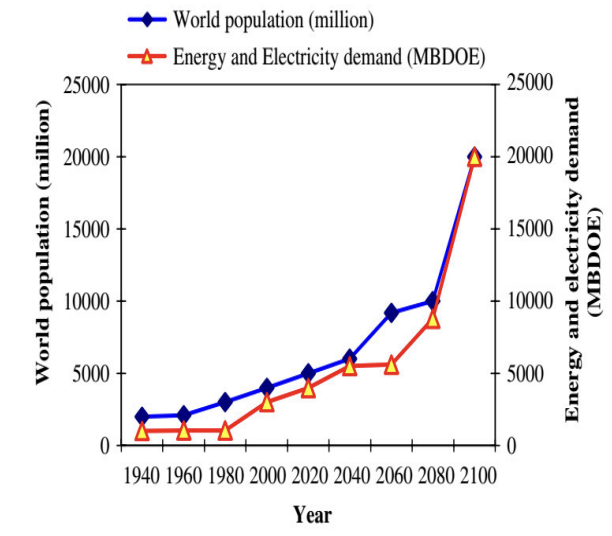
\includegraphics[width=0.85\textwidth,keepaspectratio]{media/image3.png}
\end{center}

Fuente: Review of Thermal Stress and Condition Monitoring Technologies for Overhead Transmission Lines (N. M. Zainuddin et al.)

\hypertarget{contexto}{%
\subsection{1.1. Contexto}\label{contexto}}

A escala global, la International Energy Agency (IEA, 2024) reportó que, en 2024, cerca del 80\% de los países de América Latina y Asia-Pacífico alcanzó nuevos récords de demanda pico durante una ola de calor o sufrió disrupciones importantes de la red atribuidas a eventos de calor extremo. En el plano local, el Sistema Argentino de Interconexión (SADI) refleja esta problemática global pero con una marcada agudización estacional debida al factor climático y residencial. Auditorías operativas de ADEERA señalan que la climatización residencial inyecta una exigencia extraordinaria sobre el sistema que equivale al 33\% del consumo nacional (aproximadamente 10.000 MW) en escenarios de persistencia térmica.

Los datos de operación del SADI ratifican esta profunda sensibilidad térmica. En semanas con temperaturas promedio entre 30 °C y 31 °C la potencia requerida se sostiene en una franja de entre \(27.000\text{~MW}\) y \(28.000\text{~MW}\), mientras que ante marcas térmicas templadas de 19 °C a 23 °C la demanda disminuye a niveles de entre \(17.000\text{~MW}\) y \(20.000\text{~MW}\). Esta brecha estructural superior al 30\% es atribuible principalmente a la climatización residencial.

Sin embargo, este estudio reconoce que el incremento en la exigencia energética no se distribuye de manera uniforme a lo largo del territorio nacional. Ciertas regiones exhiben una vulnerabilidad crítica debido a una combinación de asimetrías climáticas, densidades demográficas disímiles, restricciones en la capacidad de transporte local de las redes y falta de redundancia local. A este escenario se suma la disparidad en la tasa de adopción de tecnologías de eficiencia energética, como sistemas inverter o etiquetado de eficiencia clase A, y sistemas de respuesta regional que resultan insuficientes para mitigar el impacto en los nodos de distribución más exigidos del país.

A pesar de contar con una infraestructura físicamente interconectada, los partes diarios emitidos por la Compañía Administradora del Mercado Mayorista Eléctrico (CAMMESA) poseen un carácter fundamentalmente descriptivo y post-operativo. Eventos históricos de afectación sistémica, como el apagón masivo del 16 de junio de 2019 - analizado en detalle en la sección 2.3 - sumados a las auditorías de control del Estado evidencian que la falta de herramientas analíticas predictivas y la dependencia del conocimiento operativo tácito amplifican la magnitud de los colapsos. De este modo, la necesidad de transicionar desde un monitoreo reactivo hacia un modelo predictivo basado en ciencia de datos se vuelve un requerimiento prioritario para garantizar la resiliencia energética nacional.

\hypertarget{justificaciuxf3n-del-estudio}{%
\subsection{1.2. Justificación del estudio}\label{justificaciuxf3n-del-estudio}}

Pese a la relevancia creciente del problema, no se encontró publicado ningún sistema basado en datos que permita anticipar de forma cuantitativa y regionalizada aquellos momentos en que el SADI está próximo al colapso. La literatura existente aborda la estabilidad de los sistemas eléctricos desde cuatro líneas relativamente separadas: el monitoreo térmico y la evaluación de resiliencia de la infraestructura física (Zainuddin et al., 2020; Mujjuni et al., 2023), los modelos dinámicos de fallas en cascada (Dai et al., 2022; Narimani et al., 2022), el análisis puntual de eventos ya ocurridos en el SADI (Calcagno et al., 2022) y la evidencia estadística que vincula los eventos de calor extremo con las interrupciones del suministro (Liang et al., 2025; Santágata et al., 2017). El antecedente más cercano, Santágata et al. (2017), ajusta un modelo logístico de la probabilidad de interrupciones graves a partir de extremos de temperatura y de consumo, pero se circunscribe al área metropolitana de Buenos Aires y a la red de distribución. Ninguno de estos antecedentes integra variables meteorológicas y de demanda en un modelo predictivo por región del SADI que traduzca esa información en una alerta operativa accionable.

En ese sentido, este trabajo no busca corregir un modelo previo sino llenar un vacío, tratando al SADI no como un bloque único ni como regiones aisladas, sino caracterizar cuantitativamente su asimetría operativa.

\hypertarget{alcances-del-trabajo-y-limitaciones}{%
\subsection{1.3. Alcances del trabajo y limitaciones}\label{alcances-del-trabajo-y-limitaciones}}

\textbf{Alcance.} Los resultados de este trabajo están orientados a constituirse en una herramienta de apoyo a la toma de decisiones para actores vinculados a la operación y el monitoreo del Sistema Argentino de Interconexión (SADI), así como también para industrias electrointensivas que requieren garantizar la disponibilidad de potencia para su correcto funcionamiento. En una primera instancia, su aplicación concreta responde a los requisitos del Trabajo Final Integrador de la Especialización en Ciencia de Datos del Instituto Tecnológico de Buenos Aires (ITBA), con potencial de derivar en un artículo científico y, eventualmente, en el desarrollo de una herramienta piloto destinada a la industria electrointensiva nacional y áreas de gestión de riesgo eléctrico.

\textbf{Limitaciones.} Al tratarse de un trabajo individual desarrollado en el marco de un taller académico, las limitaciones responden principalmente a la disponibilidad de recursos:

\begin{itemize}
\item
  \emph{Recursos financieros}: el trabajo se desarrolla sin financiamiento institucional ni de terceros, lo que restringe el acceso a fuentes de datos pagas (por ejemplo, series meteorológicas de mayor resolución espacial, o datos de topología de red de las distribuidoras) y a infraestructura de cómputo de mayor escala.
\item
  \emph{Recursos humanos}: La investigación es conducida por un único autor, prescindiendo de un equipo interdisciplinario que incluya, por ejemplo, especialistas en ingeniería eléctrica de potencia o meteorología, quienes permitirían validar con mayor profundidad los supuestos técnicos subyacentes del modelo.
\item
  \emph{Recursos materiales}: Se trabaja exclusivamente con conjuntos de datos públicos y de acceso abierto (CAMMESA, SMN, IGN) y herramientas de software libre, sin acceso a bases de datos privadas de empresas distribuidoras ni a mediciones de campo propias. A su vez, parte del material disponible carece de la estructura o granularidad óptima para el despliegue automático de un software predictivo en tiempo real, razón por la cual el procesamiento de datos requirió técnicas de curación y adecuación manuales que podrían introducir sesgos o fuentes de error marginales.
\end{itemize}

\hypertarget{estado-de-la-cuestiuxf3n}{%
\section{2. Estado de la cuestión}\label{estado-de-la-cuestiuxf3n}}

El estudio de la estabilidad y la resiliencia de los sistemas eléctricos de potencia (SEP) ha cobrado una relevancia crítica en la agenda científica global debido al incremento sostenido de la demanda y a la mayor frecuencia y severidad de eventos climáticos extremos. La literatura especializada aborda este desafío multidimensional a partir de cuatro ejes principales: las limitaciones térmicas de la red, los modelos dinámicos de fallas en cascada, los antecedentes analíticos del caso argentino y la evidencia empírica que vincula el calor extremo con las interrupciones del suministro.

\hypertarget{monitoreo-tuxe9rmico-y-condiciones-luxedmite-de-la-red}{%
\subsection{2.1. Monitoreo térmico y condiciones límite de la red}\label{monitoreo-tuxe9rmico-y-condiciones-luxedmite-de-la-red}}

El desafío de afrontar períodos de alta carga regional no radica únicamente en la capacidad de generación bruta de las centrales, sino en la capacidad física del sistema de transporte en alta tensión para canalizar dicha energía. El límite operativo de las líneas de transmisión aérea está condicionado de forma estricta por la temperatura máxima permitida en el conductor, una propiedad físico-técnica denominada \textbf{ampacidad}.

En los conductores del tipo ACSR (\emph{Aluminum Conductors Steel-Reinforced}), que predominan en el tendido de la red troncal nacional, la temperatura máxima de diseño tolerable se sitúa en los 75 °C. Si este umbral es superado de forma sostenida debido a la combinación de una alta corriente eléctrica circulante y temperaturas ambientales extremas, la línea experimenta tres efectos degradatorios críticos:

\begin{itemize}
\item
  \textbf{Pérdida de propiedades mecánicas:} El material del conductor sufre un proceso de recocido que reduce su resistencia a la tracción y acelera el envejecimiento estructural de los activos.
\item
  \textbf{Efecto de Flechado (\emph{Sag}):} Por acción de la expansión térmica, los cables metálicos se dilatan y ceden verticalmente. Este aumento del flechado disminuye la distancia de seguridad respecto al terreno o la vegetación, elevando exponencialmente el riesgo de descargas disruptivas, cortocircuitos y arcos eléctricos.
\item
  \textbf{Reducción de los márgenes de seguridad:} El sistema de transporte se vuelve físicamente más vulnerable en el instante en que la demanda poblacional y la necesidad de resiliencia de la red alcanzan su punto máximo.
\end{itemize}

Históricamente, la operación y el despacho económico del sistema de transporte eléctrico en alta tensión se gestionó mediante el criterio de \textbf{Capacidad Estática de Línea} (\emph{Static Line Rating} o SLR). Este enfoque metodológico consiste en establecer un límite de transferencia de potencia rígido, invariable y conservador para los conductores, calculado a partir de escenarios meteorológicos teóricos y fijos para cubrir normativamente el peor escenario operacional posible (\emph{worst-case scenario}).

Como argumentan Zainuddin et al. (2020), la debilidad estructural del SLR radica en su naturaleza binaria e inflexible. Por un lado, subestima la capacidad real de transporte de las líneas en jornadas con condiciones ambientales favorables, impidiendo el despacho eficiente de energía más económica, y por el otro, sobreestima gravemente la seguridad de la red durante olas de calor severas.

En el caso del Sistema Argentino de Interconexión (SADI), esta limitación metodológica adquiere un carácter crítico. Durante los períodos estivales, cuando las marcas térmicas reales superan recurrentemente los 38 °C o 40 °C en nodos altamente exigidos, los parámetros fijos de las tablas de despacho de la Compañía Administradora del Mercado Mayorista Eléctrico (CAMMESA) dejan de reflejar el estado físico real de los activos. Al operar bajo umbrales estáticos que ignoran las anomalías climáticas dinámicas en el vano de la línea, el sistema de transporte queda expuesto a condiciones de flechado (\emph{sag}) imprevistas y desenganches automáticos por fallas a tierra, reduciendo los márgenes de resiliencia en los momentos de máxima demanda del sector residencial.

Para el caso del Sistema Argentino de Interconexión (SADI), y bajo los supuestos metodológicos de este trabajo, el análisis del riesgo se aborda reconociendo la persistencia de este paradigma estacional tradicional en los manuales de camino crítico y procedimientos de despacho históricos. Si bien a nivel sectorial e internacional se constata una tendencia hacia la investigación y el desarrollo de proyectos piloto orientados a la Capacidad Dinámica de Línea (\emph{Dynamic Line Rating} o DLR), orientados a flexibilizar los límites de transmisión mediante la integración de variables ambientales en tiempo real, su adopción masiva en lazo cerrado suele verse limitada por la alta exigencia de inversión en infraestructura de conectividad, redes inteligentes (\emph{smart grids}) y densidades de sensores de campo requeridas a lo largo de las extensas trazas de la red troncal nacional (Transener, 2024).

Ante este ecosistema técnico y regulatorio, la implementación de un modelo basado en ciencia de datos no pretende sustituir los sistemas físicos de telemedición dinámicos, sino operar como un estimador virtual complementario de la vulnerabilidad estructural. Al reconocer explícitamente la restricción en el acceso a mediciones directas de temperatura en los conductores, tal como se detalla en el apartado de limitaciones de este estudio, el desarrollo de una arquitectura analítica alimentada por variables exógenas densas (como matrices meteorológicas continuas) y variables endógenas de red (curvas de carga históricas) permite modelar probabilísticamente el riesgo de falla por región e incluso una caracterización de los nodos más vulnerables frente al estrés térmico que caracteriza al período estival argentino.

\hypertarget{fallas-en-cascada-y-modelos-dinuxe1micos}{%
\subsection{2.2. Fallas en cascada y modelos dinámicos}\label{fallas-en-cascada-y-modelos-dinuxe1micos}}

Las fallas en cascada se definen estructuralmente como una sucesión de salidas operativas de componentes vinculados de manera dependiente, donde cada desenganche individual debilita progresivamente la integridad del Sistema de Potencia (SEP) hasta culminar en apagones de gran escala. En la búsqueda de maximizar la eficiencia y reducir los costos de despacho, los sistemas modernos son operados de forma regular cerca de sus límites de estabilidad. Esta condición incrementa el riesgo sistémico de experimentar colapsos ante perturbaciones iniciales modestas. La literatura ratifica que estos fenómenos progresan mediante eventos dependientes del tiempo, tales como la sobrecarga térmica sucesiva de líneas de transmisión y la actuación secuencial de relés de protección, que pueden derivar en la fragmentación de la red en islas eléctricas aisladas, haciendo indispensable un análisis que capture la respuesta dinámica particular de cada nodo.

En sistemas con una penetración de generación renovable variable y no convencional en crecimiento, la reducción de la inercia total disponible comienza a perfilarse como un factor de vulnerabilidad crítico. La sustitución de la generación térmica tradicional por fuentes electrónicas de potencia disminuye la inercia rotatoria del sistema, restringiendo su capacidad para contener la tasa de variación de frecuencia tras una perturbación severa. Consecuentemente, los modelos tradicionales basados en el estado cuasi-estacionario (\emph{Quasi-Steady-State} o QSS) resultan metodológicamente insuficientes para predecir estos eventos, dado que omiten las dinámicas transitorias que gobiernan la propagación de fallas en redes de baja inercia.

Desde la perspectiva de la redundancia operativa, los operadores de los SEP suelen administrar márgenes de reserva de potencia para absorber desequilibrios imprevistos entre la oferta y la demanda. En el escenario eléctrico argentino, la criticidad de estos márgenes reducidos queda evidenciada de forma institucional a través del \emph{Plan de Contingencia y Previsión para meses críticos del período 2024/2026} (Resolución SE N° 294/2024), mediante el cual la Secretaría de Energía de la Nación y CAMMESA formalizaron acciones extraordinarias, como la gestión de importaciones de energía y potencia desde países limítrofes en las horas pico de los días críticos y un esquema voluntario y remunerado de gestión de demanda para grandes usuarios (GUMAs), para mitigar el estrés sistémico en jornadas de extrema exigencia térmica.

En función a lo descripto, este estudio se centra en predecir el comportamiento del sistema bajo su estado topológico actual, entendiendo que la futura integración de tecnologías de respuesta rápida, cuya viabilidad técnica y regulatoria ya comenzó a ser proyectada en el SADI mediante las convocatorias nacionales para Sistemas de Almacenamiento de Energía Eléctrica en Baterías (BESS) alteraría los supuestos de riesgo y requeriría una reevaluación de las estrategias de mitigación.

\hypertarget{el-caso-del-sadi}{%
\subsection{2.3. El caso del SADI}\label{el-caso-del-sadi}}

Retomando la asimetría regional señalada en la sección 1.1, el análisis de la resiliencia en infraestructuras críticas exige clasificar los factores que desencadenan las fallas sistémicas para determinar la viabilidad de su modelado algorítmico. Siguiendo la taxonomía internacional de la ingeniería de potencia, las interrupciones en el suministro eléctrico pueden agruparse en cinco dimensiones principales: factores externos o climáticos, tecnológicos (fallas de equipos), operativos (errores humanos y de gestión), de mercado (marcos regulatorios) e intencionales.

En la historia reciente del Sistema Argentino de Interconexión (SADI), la evidencia empírica demuestra que, si bien las perturbaciones técnicas iniciales suelen ser de origen físico o meteorológico, la magnitud final de los colapsos está frecuentemente ligada a la dimensión operativa y a fallos en los esquemas de protección automática. El apagón masivo del 16 de junio de 2019 constituye el caso de estudio nacional paradigmático de una falla en cascada, donde un cortocircuito aleatorio en la línea Colonia Elía - Belgrano escaló hasta un colapso total debido a que la Desconexión Automática de Generación (DAG) no fue reprogramada tras una modificación física en la topología de la red por obras civiles. Este antecedente expone cómo la estabilidad sistémica no depende únicamente de la infraestructura material, sino de la correcta supervisión y actualización de los flujos de información operativa.

La existencia de estas debilidades en los procedimientos de supervisión dentro de la estructura institucional argentina ha sido ratificada formalmente por el Ente Nacional Regulador de la Electricidad. En su informe de auditoría UAI 14-2024 (2025), el ENRE identificó de manera explícita la ausencia de procedimientos formales y estandarizados dentro de la División de Monitoreo de Redes. Los hallazgos del organismo de control exponen una dependencia crítica del conocimiento operativo tácito y de la pericia informal del personal de turno ante eventos de estrés. Esta carencia procedimental e institucional latente, si bien no se descarta que en el último año podría haber sido corregida parcialmente, actúa como un factor de riesgo que impediría una mitigación temprana y sistemática de los incidentes en la red troncal, propiciando que eventos de origen técnico o ambiental se amplifiquen exponencialmente debido a la falta de herramientas automáticas de anticipación.

Frente a esta realidad multicausal, es metodológicamente indispensable establecer las fronteras analíticas de este Trabajo Final Integrador. Este estudio reconoce de forma explícita que las fallas puramente operativas, los errores humanos de coordinación y las omisiones administrativas en la reprogramación de los sistemas automáticos escapan a las capacidades predictivas de los modelos de Ciencia de Datos desarrollados. Al tratarse de eventos estocásticos de carácter organizacional y conductual en momentos de crisis, el error humano no puede ser capturado matemáticamente a partir de series temporales de red.

Por consiguiente, la arquitectura predictiva de esta investigación se enfoca estrictamente en aquellas variables que sí presentan viabilidad técnica de modelado y previsión, la intersección entre los factores exógenos climáticos (estrés térmico y ampacidad) y la vulnerabilidad físico-topológica intrínseca del SADI. Al aislar el factor humano y centrar el alcance en predecir el riesgo de falla basal por nodo ante el consumo de climatización estival, este trabajo busca proveer un estimador cuantitativo objetivo. De esta forma, la analítica avanzada se postula como una herramienta de soporte orientada a detectar y mitigar los disparadores físicos de la red antes de que el sistema ingrese a la fase de propagación dinámica, donde las falencias de gestión y las vulnerabilidades de monitoreo tradicionales históricamente habrían acentuado la gravedad de los colapsos.

\hypertarget{evidencia-empuxedrica-sobre-temperatura-e-interrupciones-del-suministro}{%
\subsection{2.4. Evidencia empírica sobre temperatura e interrupciones del suministro}\label{evidencia-empuxedrica-sobre-temperatura-e-interrupciones-del-suministro}}

Más allá de los modelos físicos, una línea de la literatura cuantifica estadísticamente la relación entre el calor extremo y las interrupciones del suministro. Liang et al. (2025), a partir de registros de cortes de alta frecuencia de aproximadamente 2.800 divisiones administrativas de China entre 2019 y 2021, estiman mediante regresiones de efectos fijos que las olas de calor aumentan la frecuencia de los cortes entre 3,9\% y 4,0\% y su duración entre 7,9\% y 8,3\%. Además, cada grado adicional de temperatura durante una ola de calor incrementa los cortes en 0,1\% y cada día adicional de ola de calor, en 0,5\%. Este último resultado respalda la incorporación de variables de persistencia térmica (días consecutivos por encima de un umbral) en el modelo propuesto.

En el ámbito local, Santágata et al. (2017) analizan los eventos de temperatura extrema que afectaron al sistema de distribución eléctrica del área metropolitana de Buenos Aires entre 1971 y 2013. A partir de las desviaciones de las temperaturas máximas y mínimas y del consumo horario respecto de umbrales estadísticos, hallan que el sistema soportaba una presión comparable en olas de frío y de calor pero era mucho más vulnerable al calor (20 apagones durante olas de calor frente a tres durante olas de frío entre 2006 y 2013), y que un modelo de regresión logística binomial describe adecuadamente la probabilidad de interrupciones graves en función de los excesos de temperatura y de consumo.

Estos antecedentes respaldan la inclusión de la temperatura y de su persistencia como predictores de interrupciones. Sin embargo, ninguno de ellos aborda el caso de las regiones del SADI ni propone una alerta regionalizada para el sistema interconectado, que es el objeto de este trabajo.

\hypertarget{definiciuxf3n-del-problema}{%
\section{3. Definición del problema}\label{definiciuxf3n-del-problema}}

En consecuencia, el problema central que este Trabajo Final Integrador se propone resolver es: ¿Cómo modelar y anticipar de manera predictiva, mediante técnicas de Ciencia de Datos, la probabilidad de falla física y la vulnerabilidad diferencial de los nodos del SADI ante el estrés térmico y la heterogeneidad climática estival, transformando el monitoreo descriptivo actual en un soporte cuantitativo objetivo para la gestión preventiva del riesgo eléctrico federal?

Para abordar con rigurosidad metodológica esta pregunta central, resulta crucial resolver analíticamente la falta de una caracterización cuantitativa explícita de los cuellos de botella geográficos, la cual dificulta discriminar con precisión entre dos grandes tipologías de eventos:

\begin{itemize}
\item
  Fallas de origen estructural: Aquellas que ocurren de manera independiente de las variables climáticas, vinculadas a la degradación material intrínseca de los componentes, la falta de mantenimiento físico o eventos de vandalismo.
\item
  Fallas inducidas por estrés térmico y operativo: Aquellas que se encuentran directamente correlacionadas con los extremos de temperatura ambiente regional y el consecuente incremento en el nivel de demanda por climatización.
\end{itemize}

Esta distinción conceptual y analítica es crítica para el aporte de la Ciencia de Datos en la red debido a que las políticas de mitigación idóneas difieren en cada caso, mientras que las fallas térmicas poseen una ventana de predictibilidad que permite anticiparlas mediante esquemas de gestión de la demanda y despacho preventivo, las estructurales exigen obras de inversión de capital en infraestructura de base. Un modelo predictivo que omitiera discriminar cuantitativamente entre ambos tipos de vulnerabilidades generaría alertas poco confiables y recomendaciones operativas inespecíficas para la toma de decisiones.

\hypertarget{hipuxf3tesis}{%
\section{4. Hipótesis}\label{hipuxf3tesis}}

Lo anteriormente descripto permite a este proyecto plantear la siguiente hipótesis:

"La relación entre temperatura, demanda y falla es no lineal y heterogénea por región. En zonas de alta vulnerabilidad térmica el modelo predice bien; en zonas de falla estructural persistente, la temperatura no es el predictor relevante."

\hypertarget{objetivos}{%
\section{5. Objetivos}\label{objetivos}}

\hypertarget{objetivo-general}{%
\subsection{5.1. Objetivo General}\label{objetivo-general}}

Desarrollar un modelo predictivo regionalizado basado en algoritmos de aprendizaje automático (\emph{Machine Learning}) que estime la probabilidad de falla física en los nodos del Sistema Argentino de Interconexión (SADI) a partir de variables meteorológicas y de demanda, proveyendo un estimador probabilístico de riesgo operacional como soporte cuantitativo para la gestión preventiva estival.

\hypertarget{objetivos-especuxedficos}{%
\subsection{5.2. Objetivos Específicos}\label{objetivos-especuxedficos}}

\begin{itemize}
\item
  \textbf{Consolidar y caracterizar cuantitativamente} las asimetrías operativas y los patrones de demanda entre las distintas regiones del SADI mediante análisis exploratorio de datos (EDA), aislando el comportamiento de las fallas de origen térmico frente a las tasas de siniestralidad estructural basal.
\item
  \textbf{Identificar y parametrizar los umbrales críticos} y las relaciones no lineales existentes entre la temperatura ambiente, la demanda por climatización y la tasa de fallas por nodo, determinando los puntos de quiebre térmico específicos por región.
\item
  \textbf{Construir, entrenar y optimizar} modelos de clasificación binaria (tales como arquitecturas basadas en ensambles de árboles o regresiones logísticas regularizadas) que integren la temperatura, la carga nodal y la persistencia térmica como predictores de desenganches físicos.
\item
  \textbf{Validar el desempeño predictivo} de las arquitecturas implementadas aplicando una estrategia de separación cronológica (\emph{time-series split}) para el entrenamiento y testeo, garantizando el respeto estricto por el orden temporal de los eventos y evaluando la robustez mediante métricas aptas para clases desbalanceadas (AUC-ROC y F1-Score).
\item
  \textbf{Evaluar el valor analítico y la utilidad predictiva diferencial} del modelo a nivel federal, identificando en qué regiones geográficas las variables climáticas explican con alta precisión el riesgo y en cuáles la siniestralidad responde de manera dominante a factores estructurales no capturados por el ambiente.
\end{itemize}

\hypertarget{soluciuxf3n-propuesta}{%
\section{6. Solución propuesta}\label{soluciuxf3n-propuesta}}

Se propone el diseño e implementación de un Semáforo de Riesgo Predictivo para el SADI (Sistema Argentino de Interconexión). Este desarrollo consiste en un sistema de alerta regionalizado que, a partir del análisis multidimensional de variables de temperatura y demanda eléctrica, clasifica de forma dinámica el estado operativo del sistema en tres niveles críticos: Verde (Normal), Amarillo (Precaución) y Rojo (Crítico / Alerta).

Además de la categorización por niveles, el modelo buscará estimar probabilísticamente la ocurrencia de siniestros y fallas estructurales por región geográfica, permitiendo una toma de decisiones proactiva y mitigando el impacto de eventuales contingencias.

Para estructurar las fases de desarrollo del proyecto y garantizar la correcta gestión de los objetivos definidos, el flujo de trabajo se articulará bajo la metodología estándar \textbf{CRISP-DM} (\emph{CRoss Industry Standard Process for Data Mining}). Este marco de referencia permite organizar el ciclo de vida del proyecto de forma iterativa y coherente con las necesidades operativas del SADI, integrando la comprensión del sistema y de los datos desde su inicio hasta el despliegue final, tal como se detalla a continuación.

\hypertarget{metodologuxeda}{%
\subsection{6.1. Metodología}\label{metodologuxeda}}

La unidad de análisis fundamental está definida bajo el enfoque de día-región, considerando cada combinación única de fecha y zona geográfica del SADI. El alcance espacial contempla las regiones operativas clave del país:

NEA (Nordeste), NOA (Noroeste), Litoral, GBA (Gran Buenos Aires), Provincia de Buenos Aires, Patagonia, Cuyo, Comahue y Centro.

No obstante, esta investigación contempla una fase de experimentación y optimización de la granularidad temporal, evaluando la posibilidad de ampliar y desagregar la unidad de análisis hacia un grano más fino de hora-región, comprendiendo que esto multiplica la dimensión de la matriz, pero diluye la cantidad de eventos positivos (horas con fallas efectivas) frente a las horas de operación normal, lo que agudiza el fenómeno de desbalance extremo de clases pudiendo degradar la capacidad de generalización y penalizar las métricas de rendimiento de los clasificadores basados en ensamble de árboles (XGBoost y Random Forest).

Las fuentes de datos utilizadas son:

\begin{itemize}
\item
  CAMMESA (Informe Anual; CAMMESA, s.f.): demanda real desagregada por región, temperatura media diaria del Gran Buenos Aires (GBA), utilizada como referencia para todas las regiones en la Etapa 1, y registro histórico de siniestros no tabulados, que se deberán optimizar para el desarrollo del modelo.
\item
  Fuente de temperatura regional (a definir; por ejemplo, SMN o reanálisis ERA5): series históricas de temperatura diaria por región, a incorporar en la Etapa 2.
\item
  IGN (Instituto Geográfico Nacional): cartografía regional para el análisis de nodos.
\end{itemize}

\hypertarget{etapa-1-anuxe1lisis-descriptivo}{%
\subsubsection{\texorpdfstring{\emph{\textbf{Etapa 1 --- Análisis descriptivo}}}{Etapa 1 --- Análisis descriptivo}}\label{etapa-1-anuxe1lisis-descriptivo}}

El estudio preliminar permitió definiir tres estados operativos (Verde, Amarillo y Rojo) en función de qué tan cerca se encuentra la demanda real de su máximo histórico regional, utilizada como proxy de la carga sobre el sistema ante la ausencia de datos públicos de capacidad instalada por nodo. Los umbrales definidos son:

\begin{itemize}
\item
  Verde (Estado Normal): reserva operativa superior al 10\% del máximo histórico.
\item
  Amarillo (Alerta): reserva entre el 5\% y el 10\%.
\item
  Rojo (Estado Crítico): reserva inferior al 5\%.
\end{itemize}

Al cruzar estos estados con el registro de siniestros 2024-2025, se confirma la asimetría regional y la existencia de una tasa de falla basal diferenciada por zona:

\begin{itemize}
\item
  Estado Crítico (Rojo): tasa de falla agregada del 15,91\% --- siete veces superior a la del Estado Normal (2,35\%).
\item
  Estado de Alerta (Amarillo): tasa de incidentes del 4,0\%, zona de transición con reservas reducidas.
\item
  Estado Normal (Verde): tasa basal del 2,35\%, vinculada a factores estructurales y exógenos; engloba el 90\% de las demandas inferiores registradas por región.
\end{itemize}

Figura 2: Jerarquía de criticidad del SADI por región, según probabilidad de falla por estado operativo.

\nopagebreak[4]
\begin{center}
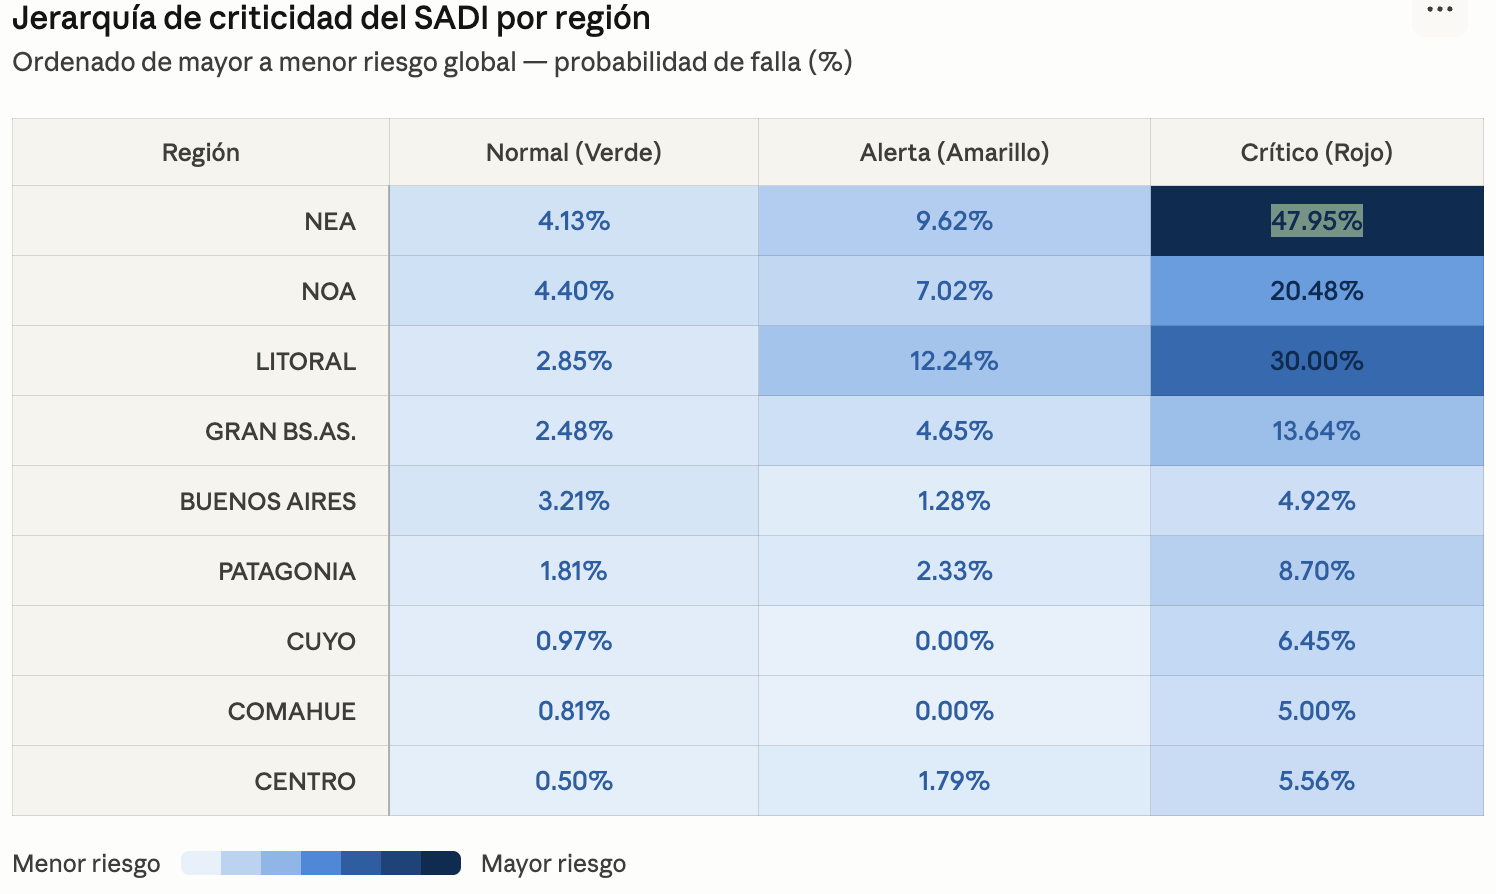
\includegraphics[width=0.85\textwidth,keepaspectratio]{media/image4.png}
\end{center}

Fuente: elaboración propia.

\hypertarget{etapa-2-modelado-predictivo-a-desarrollar}{%
\subsubsection{\texorpdfstring{\emph{\textbf{Etapa 2 --- Modelado predictivo (a desarrollar)}}}{Etapa 2 --- Modelado predictivo (a desarrollar)}}\label{etapa-2-modelado-predictivo-a-desarrollar}}

Sobre la misma base de datos se incorporarán temperatura diaria y variables de acumulación térmica (días consecutivos por encima de umbrales) para construir modelos de clasificación binaria. La validación respetará el orden cronológico (walk-forward), entrenando sobre el período más antiguo y evaluando sobre el más reciente, para evitar data leakage temporal.

\hypertarget{tuxe9cnicas-herramientas}{%
\subsection{6.2. Técnicas / Herramientas}\label{tuxe9cnicas-herramientas}}

Para resolver la tarea de clasificación binaria orientada a estimar la probabilidad de falla física e inducida por estrés térmico en los nodos del SADI, se implementará un enfoque basado en el aprendizaje estadístico supervisado (\emph{Machine Learning}) enfocado en datos tabulares distribuidos.

Dada la naturaleza infrecuente de los siniestros eléctricos en relación con los períodos de operación normal, el dataset presenta un escenario de \textbf{clases fuertemente desbalanceadas}. Por consiguiente, se descartó la utilización de arquitecturas de aprendizaje profundo (\emph{Deep Learning} o Redes Neuronales Artificiales), dado que la escasez de ejemplos positivos (eventos con fallas) incrementaría drásticamente el riesgo de sobreajuste (\emph{overfitting}) y comprometería la interpretabilidad de los predictores físicos. En su lugar, el núcleo analítico de la solución se estructurará sobre métodos basados en árboles de decisión y algoritmos de ensamble.

\begin{itemize}
\item
  \textbf{Regresión Logística:} Actuará como el modelo base inicial (\emph{baseline}). Permitirá establecer una línea de rendimiento lineal simple y evaluar si la incorporación de la complejidad algorítmica de los modelos de ensamble ofrece una ganancia real y estadísticamente significativa en la capacidad de generalización del sistema.
\item
  \textbf{Random Forest:} Se empleará como arquitectura de ensamble complementaria basada en la metodología de agregación por \emph{bagging}. Al entrenar múltiples árboles de decisión independientes en paralelo sobre diferentes subconjuntos de datos y características, este modelo destaca por su baja varianza y robustez ante el ruido. Asimismo, provee de forma nativa métricas directas de importancia de variables (\emph{Feature Importance}), lo cual resulta metodológicamente indispensable para contrastar empíricamente la hipótesis sobre en qué regiones la temperatura actúa como el predictor dominante y en cuáles predomina la siniestralidad estructural basal.
\item
  \textbf{Gradient Boosting Machines (XGBoost / LightGBM):} Constituyen la herramienta principal para el desarrollo del estimador probabilístico. Los algoritmos basados en optimización por gradiente sobre árboles de decisión construyen modelos de forma secuencial, donde cada nuevo árbol corrige los errores de predicción residuales de los anteriores. Esta técnica es óptima para capturar de manera nativa las \textbf{relaciones no lineales y los umbrales críticos de quiebre térmico} que caracterizan la demanda de climatización residencial y la ampacidad física de las líneas.
\end{itemize}

El procesamiento de datos, el análisis exploratorio estructural y la implementación de los modelos se desarrollarán bajo el lenguaje de programación \textbf{Python}, haciendo uso de su ecosistema científico estándar de código abierto:

\begin{itemize}
\item
  Pandas y NumPy para la ingesta, limpieza y estructuración espacio-temporal de las matrices de CAMMESA, el SMN y el IGN.
\item
  Scikit-Learn para las tareas de preprocesamiento, regularización lineal, balanceo de datos y cómputo de métricas de validación.
\item
  XGBoost y LightGBM para la implementación eficiente y distribuida de las arquitecturas de \emph{gradient boosting}.
\item
  Matplotlib y Seaborn para la visualización analítica de los perfiles de carga y la delimitación gráfica de los umbrales de riesgo.
\end{itemize}

\hypertarget{referencias-bibliografuxeda}{%
\section{7. Referencias-Bibliografía}\label{referencias-bibliografuxeda}}

Breiman, L. (2001). Random forests. \emph{Machine Learning} 45, 5--32. \url{https://doi.org/10.1023/A:1010933404324}

Calcagno, D. L., Cantos Cornejo, M. L., \& Baziuk, P. A. (2022). Análisis de vulnerabilidades e interrupciones del sistema argentino de interconexión. \emph{Revista Tecnología e Sociedade, 18(54),} 53--73. \url{https://periodicos.utfpr.edu.br/rts/article/view/13802}

Chen, T., \& Guestrin, C. (2016\emph{).} XGBoost: A scalable tree boosting system. En \emph{Proceedings of the 22nd ACM SIGKDD International Conference on Knowledge Discovery and Data Mining (pp. 785--794).} Association for Computing Machinery. \url{https://doi.org/10.1145/2939672.2939785}

Compañía Administradora del Mercado Mayorista Eléctrico. (s.f.). \emph{Informe Anual.} https://cammesaweb.cammesa.com/informe-anual/

Dai, Y., Preece, R., \& Panteli, M. (2022). Risk assessment of cascading failures in power systems with increasing wind penetration. \emph{Electric Power Systems Research,} \emph{211,} 108392. \url{https://doi.org/10.1016/j.epsr.2022.108392}

Ente Nacional Regulador de la Electricidad. (2025). \emph{Informe UAI Nº 14-24: División Monitoreo de Redes del Servicio Eléctrico.} Unidad de Auditoría Interna. \url{https://www.argentina.gob.ar/enre/transparencia/auditorias}

He, H., \& Garcia, E. A. (2009). Learning from imbalanced data. \emph{IEEE Transactions on Knowledge and Data Engineering,} \emph{21}(9), 1263--1284. \url{https://doi.org/10.1109/TKDE.2008.239}

International Energy Agency. (2024). \emph{How can energy efficiency alleviate rising heatwave-driven electricity demand?} En \emph{Energy Efficiency 2024}. https://www.iea.org/reports/energy-efficiency-2024/how-can-energy-efficiency-alleviate-rising-heatwave-driven-electricity-demand

Liang, J., Qiu, Y., Wang, B., Shen, X., \& Liu, S. (2025). Impacts of heatwaves on electricity reliability: Evidence from power outage data in China. \emph{iScience, 28}(2), 111855. https://www.ncbi.nlm.nih.gov/pmc/articles/PMC11848798/

Mohd Zainuddin, N., Abd Rahman, M. S., Ab. Kadir, M. Z. A., Nik Ali, N. H., Ali, Z., Osman, M., \& Mohamad Nasir, N. A. F. (2020). Review of thermal stress and condition monitoring technologies for overhead transmission lines: Issues and challenges. \emph{IEEE Access, 8,} 120784--120807. \url{https://ieeexplore.ieee.org/document/9123900}

Mujjuni, F., Betts, T. R., \& Blanchard, R. E. (2023). Evaluation of power systems resilience to extreme weather events: A review of methods and assumptions. \emph{IEEE Access, 11,} 87279--87296. \url{https://doi.org/10.1109/ACCESS.2023.3304643}

Narimani, M. R., Huang, H., Umunnakwe, A., Mao, Z., Sahu, A., Zonouz, S., \& Davis, K. (2022). Generalized contingency analysis based on graph theory and line outage distribution factor. \emph{IEEE Systems Journal, 16}(1), 626--637. \url{https://ieeexplore.ieee.org/document/9565815}

Santágata, D. M., Castesana, P., Rössler, C. E., \& Gómez, D. R. (2017). Extreme temperature events affecting the electricity distribution system of the metropolitan area of Buenos Aires (1971--2013). \emph{Energy Policy, 106}, 404--414. https://doi.org/10.1016/j.enpol.2017.04.006

Secretaría de Energía. (2024, 1 de octubre). Resolución 294/2024. Plan de Contingencia y Previsión para meses críticos del período 2024/2026. \emph{Boletín Oficial de la República Argentina.} \url{https://www.argentina.gob.ar/normativa/nacional/resoluci\%C3\%B3n-294-2024-404809}
